\documentclass[11pt]{article}
\usepackage{preamble}
\usepackage{gset}


\def\week{15}
\def\theproblem{К\week.\arabic{problem}}

\begin{document}

\setcounter{problem}{0}
\def\theproblem{Д\week.\arabic{problem}}
{\textbf{\large Дискретная математика}\hfill \textbf{(Основной поток)}

\medskip %

\textbf{Домашнее задание \week}}

\medskip

\textbf{Дайте обоснованные ответы на следующие вопросы.}


\vspace{5mm}

\p Существует ли ориентированный граф на 10 вершинах со 100 рёбрами? Если да, обязательно ли такой граф эйлеров?

Сколько ребер в полном ориентированном графе на 10 вершинах? $10 * 10 = 100$. То есть такой граф существует и он может быть только полным.
Так как существуют все ребра, то у каждой вершины исходящая степень равна 10, входящая тоже равна 10. Поэтому выполняется критерий эйлерова графа, поэтому такой граф всегда будет эйлеровым.

Ответ: Да, существует. Да, обязательно.

\p Вершины ориентированного графа~"--- целые числа от 0 до 2023. Ребро
идёт из вершины $x$ в вершину $y$ если $y-x=2$ или $x-y=3$. Найдите
количество компонент сильной связности в этом графе. 

Можно перефразировать условие так: из каждой вершины исходит ребро к второму соседу справа и 3 соседу слева, если такие есть.
Всего вершин 2024, поэтому разобъем все вершины на группы, чтобы 2024 делилось на размер группы. Возьмем размер группы равный 8.
Докажем, что 8 подряд идущих вершин - компонента сильной связности. 

\[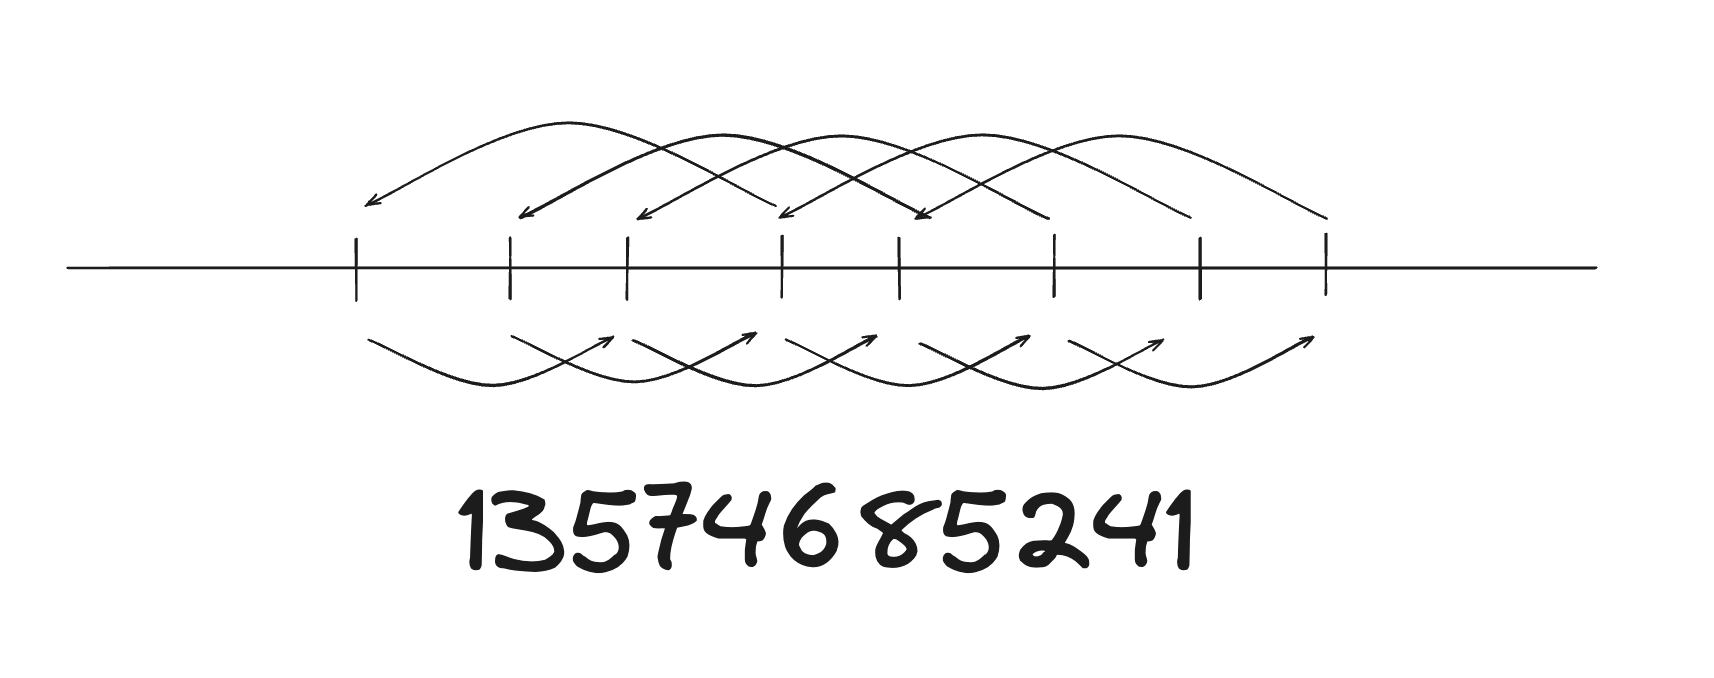
\includegraphics[width=150mm]{img}\]

Здесь я в явном виде привел цикл, проходящий по всем вершинам группы. 

Пусть мы разбили все вершины на 253 группы по 8 подряд идущих, начиная с 0. Докажем, что из любой группы можно добраться в любую другую.
Возьмем последнюю вершину в группе, тогда по ребру "вперед" \space мы можем попасть в следующую группу, если такая есть. 
Возьмем первую вершину в группе, тогда по ребру "назад" \space мы можем попасть в предыдущую группу, если такая есть. 
Поэтому если рассматривать группы, то можно записать цикл $1,2,...,252,253,252,...,2,1$.
Таким образом, можно добраться из любой группы в любую другую, значит множество всех вершин - компонента сильной связности.

Ответ: 1

\p   Функция $C\colon V\to P(V)$ сопоставляет  вершине
ориентированного графа с множеством вершин~$V$ 
область достижимости этой вершины (определение см. в задаче~\ref{Reach}). Здесь $P(V)$~"--- множество всех
подмножеств множества~$V$. Верно ли, что для
любого ациклического ориентированного графа на 2024 вершинах  функция $C$ является инъекцией?

Пусть $C$ не инъекция. Заметим, что $V \in P(V)$. Тогда если для $A \neq B \land P(A) = P(B)$, верно, что $B \in P(A) \land A \in P(B)$, значит существует путь $A \rsa B$ и $B \rsa A$, то есть в графе есть цикл. 
Противоречие. Значит $C$ - инъекция. 

Ответ: да

\p
\emph{Турниром} называется такой ориентированный граф, в котором
нет петель и для любых двух различных вершин $x$, $y$ есть ровно одно
ребро с концами $x$, $y$. 

Докажите, что любой турнир либо ациклический, либо в нем есть цикл длины 3. 

Заметим, что в турнирах нет циклов длины 1 (в турнире нет петель) или 2 (между любыми 2 вершинами ровно 1 ребро). Рассмотрим в турнире цикл минимальной длины (1). Пусть он длины больше, чем 3. Тогда возьмем 4 подряд идущих в цилке вершины. 
Назовем их $a, b, c, d$. Есть ребра $a \to b, b \to c, c \to d$. Рассмотрим вершины $(b, d)$. Если сущесвтует ребро $d \to b$, то есть цикл меньшей длины, а именно $b, c, d$, что противоречит условию 1.
Если существует ребро $b \to d$, то можно составить цикл из вершин минимального цикла, но без вершины $c$. То есть уменьшить цикл, что тоже противоречит условию 1. Таким образом, приходим к противоречию.
Значит, минимальный цикл в турнире не больше 3, но так как он не может быть размера 1 или 2, то минимальный цикл точно размера 3 (или его нет).


\end{document}
